% This is "sig-alternate.tex" V2.0 May 2012
% This file should be compiled with V2.5 of "sig-alternate.cls" May 2012
%
% This example file demonstrates the use of the 'sig-alternate.cls'
% V2.5 LaTeX2e document class file. It is for those submitting
% articles to ACM Conference Proceedings WHO DO NOT WISH TO
% STRICTLY ADHERE TO THE SIGS (PUBS-BOARD-ENDORSED) STYLE.
% The 'sig-alternate.cls' file will produce a similar-looking,
% albeit, 'tighter' paper resulting in, invariably, fewer pages.
%
% ----------------------------------------------------------------------------------------------------------------
% This .tex file (and associated .cls V2.5) produces:
%       1) The Permission Statement
%       2) The Conference (location) Info information
%       3) The Copyright Line with ACM data
%       4) NO page numbers
%
% as against the acm_proc_article-sp.cls file which
% DOES NOT produce 1) thru' 3) above.
%
% Using 'sig-alternate.cls' you have control, however, from within
% the source .tex file, over both the CopyrightYear
% (defaulted to 200X) and the ACM Copyright Data
% (defaulted to X-XXXXX-XX-X/XX/XX).
% e.g.
% \CopyrightYear{2007} will cause 2007 to appear in the copyright line.
% \crdata{0-12345-67-8/90/12} will cause 0-12345-67-8/90/12 to appear in the copyright line.
%
% ---------------------------------------------------------------------------------------------------------------
% This .tex source is an example which *does* use
% the .bib file (from which the .bbl file % is produced).
% REMEMBER HOWEVER: After having produced the .bbl file,
% and prior to final submission, you *NEED* to 'insert'
% your .bbl file into your source .tex file so as to provide
% ONE 'self-contained' source file.
%
% ================= IF YOU HAVE QUESTIONS =======================
% Questions regarding the SIGS styles, SIGS policies and
% procedures, Conferences etc. should be sent to
% Adrienne Griscti (griscti@acm.org)
%
% Technical questions _only_ to
% Gerald Murray (murray@hq.acm.org)
% ===============================================================
%
% For tracking purposes - this is V2.0 - May 2012

\documentclass{sig-alternate}

\usepackage[hyphens]{url}      % llt: nicely formatted URLs
\usepackage{todonotes}% allows to add inline comments with \todo[inline]{comment text}

\begin{document}
%
% --- Author Metadata here ---
\conferenceinfo{WOODSTOCK}{'97 El Paso, Texas USA}
%\CopyrightYear{2007} % Allows default copyright year (20XX) to be over-ridden - IF NEED BE.
%\crdata{0-12345-67-8/90/01}  % Allows default copyright data (0-89791-88-6/97/05) to be over-ridden - IF NEED BE.
% --- End of Author Metadata ---

\title{A Case Study of Using GitHub in Software Engineering Courses}

%
% You need the command \numberofauthors to handle the 'placement
% and alignment' of the authors beneath the title.
%
% For aesthetic reasons, we recommend 'three authors at a time'
% i.e. three 'name/affiliation blocks' be placed beneath the title.
%
% NOTE: You are NOT restricted in how many 'rows' of
% "name/affiliations" may appear. We just ask that you restrict
% the number of 'columns' to three.
%
% Because of the available 'opening page real-estate'
% we ask you to refrain from putting more than six authors
% (two rows with three columns) beneath the article title.
% More than six makes the first-page appear very cluttered indeed.
%
% Use the \alignauthor commands to handle the names
% and affiliations for an 'aesthetic maximum' of six authors.
% Add names, affiliations, addresses for
% the seventh etc. author(s) as the argument for the
% \additionalauthors command.
% These 'additional authors' will be output/set for you
% without further effort on your part as the last section in
% the body of your article BEFORE References or any Appendices.

\numberofauthors{1} %  in this sample file, there are a *total*
% of EIGHT authors. SIX appear on the 'first-page' (for formatting
% reasons) and the remaining two appear in the \additionalauthors section.
%
\author{
       \alignauthor Joseph Feliciano, Margaret-Anne Storey, Alexey Zagalsky\\
       \affaddr{University of Victoria}\\
       \affaddr{Victoria, BC, Canada}\\
       \email{\{noelf, mstorey, alexeyza\}@uvic.ca}\\
}
% Just remember to make sure that the TOTAL number of authors
% is the number that will appear on the first page PLUS the
% number that will appear in the \additionalauthors section.

\maketitle
\begin{abstract}
To do.
\end{abstract}

% A category with the (minimum) three required fields
\category{H.4}{Information Systems Applications}{Miscellaneous}
%A category including the fourth, optional field follows...
\category{D.2.8}{Software Engineering}{Metrics}[complexity measures, performance measures]

\terms{Theory}

\keywords{ACM proceedings, \LaTeX, text tagging}

%!TEX root = icse_seet16.tex
\section{Introduction}
%new best practices for software engineering education and training;

%focuses:
%- the contributing student
%- GH to facilitate that
%- student perceptions of the tool
%- best uses of GH

Learning about computer science and software engineering is challenging for many reasons. Students must learn the theory, but they also need to apply what they have learned to practical settings. They learn best by doing, by making mistakes, and by iterating on solutions. And because modern complex systems are not written by developers working in isolation, students need to spend a significant amount of time learning how to collaborate and coordinate with others.

Perhaps in an effort to address some of these challenges, many software engineering and computer science instructors have recently adopted GitHub for hosting their course content or handling assignment submissions. In some cases, they are using it in place of a more traditional learning management environment (such as Moodle).
%
% Peggy:  I think this paragraph is needed....  but I moved it... as not all the reviewers will know what Git or GitHub is...   Be careful it was not copied to later in the paper as Alexey suggested.  I've tweaked it a bit and reordered sentences.
GitHub is a popular social code sharing platform that leverages the Git distributed version control system (DVCS). It encourages an open workflow where collaborators can participate in a number of ways, such as contributing to discussions regarding bugs and features, or making changes to a project and allowing other collaborators to review and accept the work. Millions of people use GitHub for collaboration, and while it was originally designed for software development, there has been recent uptake in a variety of domains\footnote{\url{http://readwrite.com/2013/11/08/seven-ways-to-use-github-that-arent-coding}}.

In a previous study \cite{zagalsky2015emergence}, we investigated how and why \emph{educators} in disciplines such as computer science and statistics use GitHub. We found that they use GitHub as a learning platform because of its open workflow and transparency features, and because it offers educators the ability to reuse and remix course materials (through distributed version control), while offering their students the chance to also contribute to course materials (e.g., through \emph{pull requests}).

The educators in our study mentioned several challenges when using GitHub, notably a steep learning curve and the lack of a knowledge base of best practices around how to use GitHub in teaching. We also found that they felt it was important that their students learn how to use GitHub due to its wide use in industry, and that the open and transparent features GitHub provides would support experiential and collaborative learning in a software engineering context. However, in our first study, we neither validated these expectations nor did we gain insights into the student experience.

We now turn our attention to understanding how \emph{students} may benefit or face challenges when using GitHub in a pedagogical software engineering context. We wished to investigate whether GitHub helps students learn more effectively and if it opens up learning opportunities that the educators from our first study anticipated (e.g., peer review and easier integration of external learning resources). Such insights can help instructors that are struggling to decide if they should use GitHub in their courses, as well as guide instructors on the best ways to incorporate GitHub in an educational context. Furthermore, these insights can be beneficial to GitHub's design team (or to the designers of similar tools, such as GitLab or BitBucket) so that they can improve their tools' suitability for an educational context.

% Peggy: Cutting this next bit out, the paragraphs that were here before were quite repetitive, trying to remove that.
%In using GitHub, educators can take advantage of its open workflow and transparency features to facilitate an open, peer review process, bring in external sources of learning, and simplify the process of remixing course materials, among others. Insights from this work can determine how educators can best take advantage of these benefits, as well as helping to shape considerations towards the development of future educationally-focused tools which, similar to GitHub, gives students opportunities to contribute to the learning experience in multiple ways.
%too bias?!?


% Peggy: some of the following could fit in motivation, not sure why it is commented out here?  Am I working on the right version...
%In computer science and software engineering education, the focus has shifted from not just technical skills, but also the development of soft skills such as communication and teamwork \cite{jazayeri2004education}. One such way to develop these skills is to allow students to contribute to each other's learning experiences and to course materials \cite{falkner2012supporting}.

%This concept, called `Contributing Student Pedagogy' \cite{hamer2008contributing}, relies highly on the technology used to facilitate this learning experience.

%It is also important, however, to explore the student perspective and to discern how the use of GitHub as an educational tool might affect students.

%particularly focusing on the collaborative and contributive activities GitHub could enable students to partake in

%Conclusions from this work helped determine how GitHub-like systems can best be used in an educational context, and helped shape considerations towards the development of future educationally-focused tools which, similar to GitHub, gives students opportunities to contribute to the learning experience in multiple ways.
In this paper, we present a longitudinal case study whereby GitHub is used as a learning platform for two distinct project-based software engineering courses. We set out to investigate how GitHub impacted student learning in these courses, as well as to determine the benefits and challenges students experienced while using GitHub as part of their studies. We also gained some insights from the instructor that taught both of the courses in our investigation.

The research questions that shaped our study are:
\begin{enumerate}[RQ1]
\item How do students \textbf{benefit} from using GitHub in their courses?
\item What \textbf{challenges} do students face when GitHub is used by software engineering course instructors?
\item What \textbf{recommendations} can we give to software engineering instructors who wish to use GitHub for teaching?
\end{enumerate}

% Peggy: this next paragraph is quite repetitive too, as Cassie suggests it could go in the abstract.
% NF: Commenting out for now, re-adding to abstract when I get there tomorrow afternoon
% The findings from our case study indicate that software engineering students do benefit from GitHub's transparency features and open workflow. However, students were concerned that since GitHub is not inherently an educational tool, it lacks key features that prevent it from being an ideal tool for this context. Moreover, we highlight the importance of tool literacy and of educating both students and instructors about GitHub's features and workflow, to create an environment that maximizes its benefits in software engineering education. We are just at the start of this adoption curve, so it is important to understand the opportunities and risks using GitHub may introduce to the teaching of software engineering and computer science.

%cse and seet, shift towards more real life skills gained through PBL, CSP, etc.

%git, github, vc being used in classes

%issues in learning tools?

%why do I talk about CSP? because of its potential for that need. Haaranen -> contributing to course material

%!TEX root = icse_seet16.tex
\section{Background}
The use of software tools to support learning, teaching, material dissemination, and course management is an important aspect of education, regardless of the domain. In the following, we first provide some background on Learning Management Systems (LMS) and research on how students learn through contributions. This is followed by a description of GitHub and an overview of research related to how GitHub-like tools have been used in education.

\subsection{The Evolution of Learning Management Systems}
Traditionally, university educators employ the use of LMSes to manage the courses they teach. An LMS provides students and educators with a set of tools for typical classroom processes. LMSes such as Blackboard, Moodle, and Sakai provide instructors with a variety of features for organizing and administering courses, including file management, grade tracking, assignment hosting, and discussion rooms \cite{kumar2011comparative}.

In addressing common features in LMSes, Malikowski \emph{et al.} \cite{malikowski2007model} developed a model that distinguishes LMS tool features into five categories: (1) transmitting course content, (2) evaluating students, (3) evaluating courses and instructors, (4) creating class discussions, and (5) creating computer-based instruction. Their research showed that the most prominent use of an LMS is to transmit information to students, whereas features for creating class discussions and evaluating students saw moderate to low-to-moderate usage, respectively.

With the rise of Web 2.0 and `the social Web', LMSes have become more social and collaborative. For example, Edrees \cite{edrees2013elearning} compares the `2.0' tools and features of Moodle and Blackboard, two of the more popular LMSes, identifying that they both now include social features such as wikis, blogs, RSS, podcasts, bookmarking, and virtual environments. Despite the popularity of these features, many researchers and educators have expressed concerns about using traditional LMSes to incorporate and emphasize student participation. McLoughlin \cite{mcloughlin2007social} believes that participatory learning lends itself well to education as students are provided with more learning opportunities where they can connect and learn from each other. However, he notes that while there were signs that Web 2.0 tools could make learning environments more personal, participatory, and collaborative, LMSes tend to be more focused on administration tasks than on the learner. Dalsgaard \cite{dalsgaard2006social} also points out the weaknesses of LMSes for supporting learner-centered activities such as independent work, reflection, construction, and collaboration, arguing that students should be provided with a myriad of other tools to support such activities.

\subsection{The Contributing Student}
Computer science and software engineering education has started embracing a pedagogy that not only focuses on technical skills, but also on soft skills such as communication and teamwork \cite{jazayeri2004education}. One way to develop these skills is to allow students to contribute to each other's learning experiences \cite{hamer2006some}. This concept, which Hamer calls a Contributing Student Pedagogy (CSP) \cite{hamer2008contributing}, is formally defined as: \textit{``A pedagogy that encourages students to contribute to the learning of others and to value the contributions of others.''} It relies on technology to facilitate the learning experience, where the learning tools typically support activities such as peer review, content construction and solution sharing, amongst others.

There are various characteristics of CSP in practice: (a) the people involved (students and instructors) switch roles from passive to active, (b) there is a focus on student contribution, (c) the quality of contributions is assessed, (d) learning communities develop, and (e) student contributions are facilitated by technology. Falkner and Falkner \cite{falkner2012supporting} observe the benefits of incorporating student contributions into their curriculum, such as increased engagement and participation, and the development of critical analysis, collaboration, and problem solving skills---important skills for a computer scientist or engineer.

\subsection{GitHub-style Systems in Education}
GitHub is one such technology that shows the ability to support certain CSP activities. In particular, it provides several features that aid collaboration and support user contributions. Users can make changes to other people's work in separate repositories or branches, and they can make a \emph{pull request} to invite the original repository owner to review and \emph{merge} their changes into the base version of the software repository. Issue tracking allows contributors to discuss any aspect of a project, including bugs, feature requests, and documentation \cite{bissyande2013got}. Moreover, GitHub's openness and transparency features, which allow users to easily see all activities inside a repository or from a user they're following, fosters both direct and indirect collaboration \cite{dabbish2012social}.

Haaranen \& Lehtinen \cite{haaranen2015teaching} conducted a case study where Git and GitLab (an open source platform similar to GitHub) were used in a large computer science course. Students could contribute to the course material by making corrections via \emph{pull requests}. The authors discussed that the ability to perform pull requests is an essential industry skill.

The educators we probed in our previous study~\cite{zagalsky2015emergence} described how using GitHub's transparency features in their courses allowed them to encourage student participation. Moreover, \emph{diffs}, issue tracking, and merge requests in GitHub provide support for code reviews \cite{kalliamvakou2014promises}, a peer-review process that promotes a positive student attitude towards work, as well as training in critical reviewing and communication skills \cite{hundhausen2013talking}.
%NFTODO: discuss more of last study

Kelleher \cite{kelleher2014employing} documented his process of using GitHub in the classroom, describing how the transparency of activities alerted him to possible acts of plagiarism and how the integrated issue tracking could be used for annotating code. Griffin \& Seals \cite{griffin2013github} leveraged Git's \emph{branch} and \emph{merge} features to simplify assignments and submissions, however, they felt that GitHub's `social coding' platform might not suit standard programming assignments that need to remain private. These studies follow early examples of an educational use of other version control tools, such as Concurrent Version Control (CVS) \cite{reid2005learning} and Subversion \cite{clifton2007subverting}. In most of these cases, the tools were used for assignment submission, to simplify the management of courses, and to allow students to collaborate with less effort.

%!TEX root = icse_seet16.tex
\section{Methodology}
%CASE STUDY
Since we previously studied the use of GitHub by educators from various disciplines \cite{zagalsky2015emergence}, we turned to investigate student perspectives on the suitability of GitHub for supporting their education. We focused on how students feel GitHub can benefit their learning and the challenges they may meet in using such a tool as part of their education. To gain insights on our research questions, we conducted a case study \cite{yin2013case,runeson2012case} where we drew from multiple sources of evidence---interviews and a survey---to investigate the potential of using GitHub for post-secondary computer science and software engineering courses. The research questions addressed in this work include:

% We used a qualitative approach to study the student perspective of GitHub use in education. As Creswell \cite{creswell2013research} suggests, a qualitative and exploratory approach best suits research when a concept or phenomenon requires more understanding because there is little pre-existing research. Yin \cite{yin2013case} introduces case studies as \textit{``an empirical inquiry that investigates a contemporary phenomenon within its real-life context, especially when the boundaries between phenomenon and context are not clearly evident.''} Case study design, according to Yin, should be used when the study is focused on the natural behavior of participants and when the context is important for the study. Because these conditions apply to the nature of the research questions asked in this study, we chose the case study design for this work. Specifically, the study was exploratory, serving as an early investigation on the student perspective of using GitHub in the classroom and to potentially build new theories or derive new hypotheses \cite{easterbrook2008selecting}.
%
% Specific to software engineering, Runeson \cite{runeson2012case} defines case studies as \textit{``an empirical enquiry that draws on multiple sources of evidence to investigate one instance (or a small number of instances) of a contemporary software engineering phenomenon within its real-life context, especially when the boundary between phenomenon and context cannot be clearly specified.''} In this work, we aimed to draw from multiple sources of evidence---students and instructors, interviews and a survey---to investigate the potential of using GitHub for post-secondary computer science and software engineering courses. It's important to learn student perspectives in this context and to explore the suitability of GitHub for supporting education.

\textbf{RQ1: How do students benefit from using GitHub in their courses?} We've seen evidence that GitHub can benefit educators in a number of ways \cite{zagalsky2015emergence} and that they believe GitHub helps their students. We wished to validate these educator impressions, but also reveal student perceptions of how GitHub and its workflow may benefit them.

\textbf{RQ2: What challenges do students face when GitHub is used by software engineering course instructors?} When adopting a new tool for a course---particularly a tool not tailored towards education---there may be some friction involved or a variety of other challenges. We aimed to identify these issues to alert educators using GitHub in their courses.

\textbf{RQ3: What recommendations can we provide software engineering instructors who wish to use GitHub for teaching?} Just as there are a variety of ways to use GitHub for development purposes, an educator also has many options for using GitHub in their courses. We provide recommendations to future software engineering instructors wanting to use GitHub to support their courses based on insights from students as well as relevant literature.

\subsection{The Case Study}
For this study, we were opportunistic in finding cases and sought instructors who could and were willing to try using GitHub. We were fortunate to recruit a university instructor who wanted to try using the tool in two different software engineering courses offered in the same semester: a Distributed Systems (DS) course aimed at both undergraduate and graduate students, and a Software Evolution (SE) course for senior undergraduate students. The DS course covered topics surrounding distributed systems and included concepts such as design considerations, fault tolerance, and cloud computing. The SE course covered the development of large-scale systems and how software evolves due to the many individuals that have a part in developing it over its lifetime.

Both classes were similar in size (29 in SE and 34 in DS) and in learning activities (weekly labs and two course projects). The course projects involved individual programming or collaboratively working with others (in groups of 2-4 students) to produce a project relating to the course topic: in the DS course, building systems that involve multiple computational devices, and in the SE course, evolving existing systems or utilizing them to create new ones.

Projects were open-ended and students could choose what they created, what topics they addressed, and what technologies and languages they utilized. Students were required to make their work publicly available so that other people, both inside and outside the course, could view their projects. The overwhelming majority of students opted to use GitHub to host their projects. The instructor did not formally introduce GitHub to the students, so those unfamiliar with the tool had to learn from others or teach themselves.
% Peggy: why is this commented out? NF please check.
% Noel: I didn't think this was necessary to add (an unimportant detail)
 %The course instructor for both courses informed them that course materials were to be hosted on GitHub, and during the first laboratory session, students had to create GitHub accounts if they did not already have one.

\subsection{How GitHub Was Used During the Case Study}
Despite being relatively unfamiliar with GitHub and its features, the course instructor opted to utilize GitHub in the same way for both courses, using its features in three pivotal ways: material dissemination through the course repository, lab work through the `Issues' feature, and project hosting in students' repositories. The advanced use cases other instructors described in our previous study \cite{zagalsky2015emergence}, such as utilizing pull requests for assignment submissions, were not used for these courses. The main course instructor was aware of some of these features but was not comfortable using GitHub beyond their knowledge.

The main use of GitHub was for material dissemination: the instructor hosted a public repository which all students could access to find the work they had to do for any given week. The instructor updated this repository weekly, adding lab assignments, links to readings, and the student homework for the week. All of the content was organized into a calendar-style table made with Markdown and was posted on the home page of the course repository. If students wanted to make changes to the content, they could `fork' the repository and use a Pull Request to alert the instructors, although the instructor did not emphasize this feature during the courses.
%\todo[inline]{CP: is the fact that it wasn't advertise actually significant? if not, I'd remove that bit. also, did the students even make use of it? I thought no one did, but I can't remember anymore.}
% NF: In this case, yes. Some students used it but others didn't, and a few said that she should have advertised it a little more

The other main use of GitHub was for hosting lab content and related discussions. The courses contained labs---2-3 hour long sessions once a week---in addition to the regular lectures, which often involved researching a topic and reporting results, or giving other groups feedback on their projects. Using each course repository's `issues' page, a dedicated issue was created for each lab, similar to a forum post, and students made comments on the appropriate issue based on their lab work. Students were free to work in groups, and when commenting on an issue, would \emph{`@mention'} their group members to indicate who the respondents were.

GitHub was also used for students to host their individual or group project work. Although students were not mandated to use GitHub for their projects, most work was hosted on GitHub in individual repositories. These repositories were publicly available so others in the course could view the work and give feedback.

%\footnote{\url{https://moodle.org/}}
In addition to GitHub, the course instructor opted to use a version of the Moodle LMS. Moodle generally allows instructors to make their course content available for students to access and interact with, enable communication between the instructors and students through forums, post quizzes, create wikis for a class to edit, and track student progress and performance. Moodle is a closed environment that is invite-only and, unlike GitHub, has the capability of having artifacts that are private not just from the public but from other participants as well. For the courses in our study, Moodle was used for artifacts that the course instructor felt should not be publicly available, including student grades and student responses to the course readings.
%\todo[inline]{CP: should you talk a little more about how Moodle allows one to control privacy/access better?}

\subsection{Research Methods}
We recruited student participants using a sign-up sheet during the first week of each course. Participation was voluntary and students who signed up were not required to participate in all phases of the study---those who were interviewed did not necessarily respond to the subsequent validation survey (discussed below).

The first phase of the study consisted of interviews with the students. Most interviews were one-on-one, however, due to scheduling reasons, some students requested to be interviewed in groups of two or three. Interviews lasted 20-30 minutes and were conducted face to face in a meeting room. Audio from every interview was recorded with participant consent and notes were taken for reference. The interviews were semi-structured based on 12 guiding questions\footnote{\url{https://goo.gl/oszl17}} and we probed further with additional questions as needed to gain their insights. We also interviewed the instructor of the courses at the end of the semester to get further understanding on how GitHub supported their teaching. This supported the exploratory nature of our research questions and supported the discovery of interesting insights.
%TODO: footnote

%\todo[inline]{I don't have this in findings yet, because I'm not entirely sure the instructor stuff adds enough to the paper, %Peggy: since it is not a question I think it is perhaps ok to leave it out but it may be nice to have some of this in discussion to add to the previous study}
%We also interviewed the instructors---the professor and the lab instructors (one for each course)---towards the end of the semester in order to find out how they utilized GitHub in their labs and to uncover their opinions on the tool's effectiveness towards the learning activities they engaged in with their students. These interviews followed a similar format to those with the students: semi-structured, 20 minutes long, with approximately 7 guiding questions. These interviews provided additional context for understanding the responses we received from the students.

In a second phase, we conducted a survey with the students to validate our findings and to confirm or contradict the themes that emerged from our analysis of the interview data in phase one.

\subsection{Data Collection and Analysis}
We conducted interviews with 12 students from the SE course, 6 students from the DS course, and one student who was taking both courses, for a total of 19 interviews.
To give students sufficient experience with GitHub, these interviews occurred no earlier than 7 weeks after the start of the semester and all were concluded within 5 weeks.

 The main distinction between the two courses was that SE was an undergraduate course whereas DS had a mix of undergraduate and graduate students. Otherwise, the courses were laid out in a similar manner (as outlined in Section 3.2). Table \ref{table:interviews:students} summarizes the previous experience the interviewed students had with GitHub.

\begin{table}[h]
    \vspace{-10pt}
        \caption{Participants and their prior experience with GitHub.}\label{table:interviews:students}
    \vspace{-10pt}
    \begin{center}
        \begin{tabular}{c | c | c}
            \hline
            ID & Prior GitHub Experience & Degree Type \\
            \hline
            DS1 & Inexperienced & Graduate \\ \hline
            DS2 & Used Academically, Professionally & Graduate \\ \hline
            DS3 & Used Academically, Professionally & Graduate \\ \hline
            DS4 & Inexperienced & Graduate \\ \hline
            DS5 & Used Academically & Graduate \\ \hline
            DS6 & Used Academically & Graduate \\ \hline
            SE1 & Used Academically, Professionally & Undergraduate \\ \hline
            SE2 & Inexperienced & Undergraduate \\ \hline
            SE3 & Used Professionally & Undergraduate \\ \hline
            SE4 & Inexperienced & Undergraduate \\ \hline
            SE5 & Used Personally & Undergraduate \\ \hline
            SE6 & Used Academically & Undergraduate \\ \hline
            SE7 & Used Professionally & Undergraduate \\ \hline
            SE8 & Inexperienced & Undergraduate \\ \hline
            SE9 & Used Professionally & Undergraduate \\ \hline
            SE10 & Used Casually & Undergraduate \\ \hline
            SE11 & Used Professionally & Undergraduate \\ \hline
            SE12 & Used Academically & Undergraduate \\ \hline
            SE13 & Used Academically & Undergraduate \\ \hline
        \end{tabular}
    \end{center}
    \vspace{-12pt}
\end{table}

We transcribed every interview and coded the responses using a content analysis methodology~\cite{charmaz2006constructing}.
We labeled segments according to the research questions of the study, and from these codes, we iteratively identified themes and concepts that surfaced multiple times. After grouping the themes into well-defined categories, we compiled a final list of themes. To check for biases, the coding of the interviews was reviewed by another researcher. To reduce possible biases, as themes emerged, we also searched for and reported counter examples to the findings (some of these counter examples are discussed in a thesis due to space constraints in this paper~\cite{feliciano2015towards}). Furthermore, the themes that emerged from the interviews with students were validated through the survey and the interviews with the instructor.
%\todo[inline]{NF: Add citations here, longer, add a reference to your thesis, Peggy:  I addressed this a bit add, the charmaz to the references NF and check it is correct, also add a reference to your thesis}
% Noel: Done, keeping comment in case I missed something

The validation survey in the second phase of our research was distributed during the final lab session of each course and students were asked to anonymously fill out an online form with details about their experiences. As mentioned above, survey respondents did not necessarily participate in the interview phase. We received 18 student responses from the DS course (4 of which were interviewed) and 15 responses from the SE course (9 of which were interviewed), for a total of 33 responses.

%opportunistic
%group interviews
\subsection{Limitations}
There are a number of limitations with our research design that we mention here.
%Internal validity concerns biases that might affect the results of a study \cite{creswell2013research}.

Our decision to recruit an instructor that had not used GitHub before (either for other work or for teaching) may have influenced (negatively) the experience of the students we wished to study. We made this decision as our previous research on this topic had gathered perspectives from instructors that generally knew GitHub quite well.

The recruitment methods we used to engage students may have resulted in biased opinions, as the students that were willing to be interviewed or surveyed may have been students who felt strongly about GitHub (positively or negatively), whereas those without a strong opinion may have chosen not to participate. By interviewing many students, however, we were able to uncover contradictions or discrepancies between the opinions we gathered. We also tried to offset this limitation by including a validation survey in our design, which had a reasonable response rate of 53\%.

We also recognize that the questions we asked in the interviews and in the surveys may have been biased. In an attempt to limit this as much as possible, we piloted the questions and had members outside our team review them for biases.

When we coded the interviews, only a single coder was involved, but we had an expert reviewer question the themes that emerged and review the coding for potential biases and inconsistencies. We further validated the emergent themes by interviewing the instructor, and by hosting a validation survey. Finally, we reported discrepant information---in the interviews and between the interview and survey data---to illustrate that not all students shared the same opinions.

Finally, we recognize that the findings from this single case study cannot be generalized to other settings~\cite{runeson2012case} where GitHub may be used in software engineering courses. We tried to offset this by asking the instructor to use the tool in two different courses. One particular issue that we alluded to above was the instructor's lack of experience with GitHub. This may have influenced our results, but in a negative way, as the instructor was not able to give more guidance to the students using the tool. However, many of the findings we report are reflected in other studies that use similar tools for classes, such as Kelleher's study on Git and GitHub \cite{kelleher2014employing}, and Haaranen and Lehtinen's study on Git and GitLab \cite{haaranen2015teaching}.

\section{GitHub Use}
This section describes the courses used in the case study and details GitHub and how it was used as a platform to support learning and teaching.

\subsection{Courses}
The two courses were a computer science (CS) course aimed at both undergraduate and graduate students, and a software engineering course (SE) that was only taken by undergraduate students. Both classes were similar in size (30-40 students) and in learning activities (weekly labs and two course projects). The course projects involved programming individually or collaboratively working with others (in groups of 2-4 students) to produce a project relating to the course topics - in one case, projects relating to the use of existing software systems to create new ones and in another, projects relating to building systems that involve multiple computational devices.

Projects were open-ended with regard to what the students created, what topic they address, and what technologies and languages they utilize for building. However, student work was required to be publicly available so that other people, both inside and outside of the course, could view their projects. The overwhelming majority of students opted to use GitHub to host their projects. However, there was no formal introduction of GitHub to the students. The course instructor for both courses informed them that course materials were to be hosted on GitHub, and during the first laboratory session, students had to create GitHub accounts if they did not already have one. Otherwise, students were left to teach themselves and each other, or ask questions to their lab instructors should they have any.

\subsection{GitHub Use in the Course}
The course instructor opted to utilize GitHub in the same way for both courses, using its features in three pivotal ways: material dissemination through the course repository, lab work through the `Issues' feature, and project hosting through various repositories. The advanced use cases we discussed in Chapter 4, such as utilizing pull requests and assignment submissions, were not used for these courses. The main course instructor was aware of some of these features but was not comfortable using GitHub beyond their knowledge.

% \begin{figure}[h!]
%  \caption{The front page of the SE Course Repository---the course schedule}
%  \centering
%    \includegraphics[width=0.8\textwidth]{schedule}
%  \label{fig:schedule}
% \end{figure}

The main use of GitHub was for material dissemination: the instructor hosted a public repository which all students could access to find the work they had to do for any given week. The instructor would update this repository weekly, adding lab assignments, links to readings, and the student homework for the week, as seen in figure \ref{fig:schedule}. All of the content was organized into a calendar table made from Markdown, and it was visible on the home page of the course repository as a `readme' file. Students could `fork' the repository to request changes to be made if they wished, though this possibility was not advertised to the students explicitly.

The other main use case was in the repository's `issues' page, where all labs (2-3 hour long sessions once a week in addition to the course lectures) were hosted. These labs would often involve researching a topic and reporting results, or giving other groups feedback on their projects. A dedicated issue would be created for each lab, similar to a forum post, and students would then make comments on these issues based on their lab work. Students were free to work in groups, and when commenting on an issue, would `@mention' their group members to indicate who the respondents were.

GitHub was also used for project hosting. Although students were not mandated to use GitHub for their course projects, most projects were hosted on GitHub in individual repositories. These repositories were public so others in the course could view the work and give feedback.

In addition to GitHub, the course instructor opted to use CourseSpaces\footnote{\url{https://www.uvic.ca/til/services/services_cs/index.php}}, a version of the Moodle LMS\footnote{\url{https://moodle.org/}}. CourseSpaces generally allows instructors to make their course content available for students to access and interact with, to enable communication between the instructors and students through forums, to post quizzes, create wikis for a class to edit, and to track student progress and performance. For these courses, CourseSpaces was used for work that the course instructor felt should not be publicly available. For example, student grades were hosted on CourseSpaces, as well as student responses to the course readings as the course instructor felt that their potential criticisms needed to be private.

%!TEX root = icse_seet16.tex
\section{Findings} % (fold)
\label{sec:Findings}

% Noel: Not sure why this is commented out, we need some preamble and this seems as good as any
We present the findings according to our research questions, and highlight the main themes that emerged alongside representative quotes from the interviews.
%Each participant quote will be identified depending on which course they were taking, as seen from Table \ref{table:interviews:students}. Before that, we provide some insights how GitHub was used in the courses in our case study.

\subsection{Student Benefits of Using GitHub for Software Engineering Courses}
Previous work~\cite{zagalsky2015emergence} has shown that GitHub introduces numerous and sometimes surprising advantages in the context of learning and teaching, however, it is important to consider how this is perceived by the students involved. Our study reveals emerging themes pertaining to the benefits of using GitHub in education from the student perspective.

%In this section, we discuss the benefits that emerged from the students' perspectives from the three main uses of GitHub in their courses: for schedule and material dissemination, for discussions, and for hosting their project work.  %Many of these benefits stem from GitHub being a tool commonly used in industry, as well as from the advantages that Git offers for managing individual and group work.

\textbf{Benefit: Gaining and Demonstrating Industry-Relevant Skills and Practices}\\
To succeed in modern software development, students need to be familiar with best practices (e.g., peer review, cross-team collaboration) and commonly used tools (e.g., continuous integration tools, distributed version control systems). Many of the interviewees [SE2, SE3, SE4, SE5, SE6, SE7, SE8, SE11, SE13, DS4] mentioned that using GitHub in their courses provided a good introduction to the tool and to relevant practices. \textit{``I think when you go and work in software development too, you should get used to [having] lots of eyes being all over your work; that's just the way it's gonna be, so it's practice before real life.''} [SE8]

% Students came into the course with varying degrees of experience with GitHub, as shown on table \ref{table:interviews:students}. Five interviewees had minimal or no experience using it, while others were very knowledgeable about the tool, either through their own uses, through group projects for other classes, or through co-op jobs. Many, at least those who attended the University of Victoria for the majority of their undergraduate studies, had some experience with Subversion, a different version control tool that is taught in a second-year course.

% Many of the interviewees mentioned that using GitHub in class provided a good introduction to the tool for them, even with just the basic use of GitHub to manage course activities such as material dissemination and discussion: \textit{``I think it's pretty good. I mean one thing is that because I'm using it in class, it's made me learn the tool \ldots and that's where the big takeaway is: that I've been able to transfer those skills, I've done some other projects just on my own time using GitHub.''} [SE2]

% For the most part, students who supported this theme believed that the use of GitHub for their courses and projects helped them experience a style of collaboration that they will encounter often in their careers. In comparison to the use of more traditional LMSes, one student noted why using GitHub might be advantageous for them: \textit{``Well, I like how it's the bonus of more practice of something you're gonna use in industry, whereas none of us are gonna use CourseSpaces or Connex when we're out on a co-op or out on a job.''} [SE3]

% Importantly, however, putting their projects on GitHub provides practice for real-life scenarios. SE8 describes why it was beneficial to have their work publicly available for both classmates and outsiders to see: \textit{``I think when you go and work in software development too, you should get used to [having] lots of eyes being all over your work; that's just the way it's gonna be, so it's practice before real life.''} [SE8]

% Beyond the benefit of using GitHub in programming projects, which is what it was designed for, the basic use of GitHub to manage course activities such as material dissemination and discussion was also beneficial to students as an introduction to the tool, with some caveats. \textit{``It's a good introduction to GitHub as a platform; it might not be a good introduction to Git as a tool. Because there's a lot of wizardry that you can do with Git that you'd never learn just doing what we did here \ldots but definitely a good start to get people using Git.''} [SE11]

Despite previous experience with the tool, using GitHub in their courses introduced some students to specific features that they were not necessarily aware of, features they believe are important to learn. \textit{``This is the first time I've actually used the issues portion of GitHub.''} [SE13] Even with the most basic use of GitHub in a course (material dissemination), students were able to reap the benefit of being exposed to a tool widely used in industry.

% Out of all the benefits described by students, the benefit of getting an introduction to GitHub and its features was talked about the most, as [SE2, SE3, SE4, SE5, SE6, SE7, SE8, SE11, SE13, CS4] specifically mentioned this benefit. The importance of this benefit is further emphasized by these students asserting their intention to continue using GitHub or to use GitHub even more after the course ends. This benefit was shared by students irrespective of their prior experience with GitHub. \\

% \textbf{Benefit: GitHub as a Portfolio} \\
% Many students believed that using GitHub to host their course projects will be beneficial to them in the future. These students described that hosting their code from other courses or from personal projects on their GitHub accounts benefited them in various ways. For example, SE5 organized their code on GitHub for easy access when helping friends: \textit{``I know that when you're trying to help somebody out, you can always just say `Check out my GitHub', I know I've done that with a few of my buddies \ldots and I don't have to search through my files, it's just on GitHub, and you look on there. It's a good organization tool.''}
%
Another important aspect of the use of GitHub is the current concept of mutual assessment~\cite{Singer2013} and the ability to use the tool as part of one's portfolio. Interviewees [SE5, SE6, SE7, SE8, SE11, SE13, DS3, DS4] mentioned the importance of publicly presenting their work on GitHub. It is not uncommon for employers nowadays to refer to GitHub for hiring purposes\footnote{\href{http://www.cnet.com/news/forget-linkedin-companies-turn-to-github-to-find-tech-talent}{http://www.cnet.com/news/forget-linkedin-companies-turn-to-github-to-find-tech-talent}}. In fact, some of the students we interviewed had already been contacted by potential employers who wanted to view their GitHub accounts: \textit{``I think all three companies that I applied to this semester wanted me to link to my GitHub. So I was really lucky that I had [a class] project on there. And I think when this [course's] project is done too, it'll also be really nice to have up there, after we clean it up.''} [SE6]

% CS2 also shared that interviewers inspected their code during an interview, highlighting the importance of having functional code in one's GitHub account: \textit{``These days I see that employers also want to see your GitHub page. While I was giving an interview for my coop, he did actually go into my GitHub profile and try to compile some of my code, so they do want you to have some online presence on GitHub.''}

%\textit{``Well I believe it's good for future employers. I remember I put directly on my resume saying you can check out the work I've done on GH. I included the link right on there and every person I handed my resume to were just like \'hey, fantastic!\' \ldots it's a good way to get your skillset out there.''} [SE5]

%The ability for students to use GitHub as a portfolio where they can show off their projects to potential employers was, for many, an important benefit of using the tool. There were students who were introduced to GitHub as part of their course, but knew the importance of having work on GitHub. This benefit motivated some students to continue putting their work on GitHub.
% The benefit of using GitHub as a portfolio was shared by [SE5, SE6, SE7, SE8, SE11, SE13, CS3, CS4]. \\

\textbf{Benefit: Enabling Cross-Team Collaboration and Contributions}\\
%In these courses, projects were open and visible to other students, creating opportunities for student contribution, a workflow that GitHub encourages. This was demonstrated by a student's group getting feedback from and providing feedback to others: \textit{``For instance, one [issue] was our script wasn't taking in command line arguments if there were spaces in them properly. And then someone [gave us a suggestion that we used]. And then to be able to see what other people are having problems with and give suggestions.''} [SE3]
Requiring students to host their course projects openly on GitHub and the heavy reliance on GitHub in the course resulted in students looking at and contributing to the work of others. Students provided feedback and received suggestions from others [SE2, SE3, SE5, SE7, SE10, SE11, SE12, SE13]. And while some lab assignments required students to look at the work of other students, many students reported that they would often peruse other projects outside of the requirements. In a few cases, students utilized code that other groups built, and as a result, helped them discover and fix issues in the original code. \textit{``I believe that one other group decided for project 2 to use [our project 1] and they made a couple of Pull Requests I think.''} [SE10]

By facilitating student contributions and cross-team collaboration, the use of GitHub enabled a participatory culture~\cite{jenkins2009confronting} where students openly created and remixed content and felt their contributions mattered. As a result, GitHub encouraged peer review practices among students: \textit{``I thought [peer reviews] was the best way to learn actually \ldots It forced you to put yourself in a position where you have to defend what you did, which I think is good for quality because you have to actually care.''} [SE11] The use of GitHub also provided collaborators in group projects an easy way to track and keep up with each other's work: \textit{``You can see exactly what the other person has contributed, and you can look it up again a month later \ldots then it's a good way to keep accountable. And it's good for yourself too, because you know they can see your work, so you wanna make sure that it's top notch and easily readable.''} [SE5]

%The ability to open up student work to anyone simplifies the peer review process, particularly with the `social coding' emphasis of GitHub where others can make inline comments or corrections themselves.

% Helping other projects, either through discussion or through collaborating on the code, offered students new ways to participate that are unique to GitHub and similar types of systems. Students effectively collaborated with each other with the aim of producing better work, as was noted by [SE2, SE3, SE5, SE7, SE10, SE11, SE12, SE13]. \\

%\textbf{Benefit: Keeping Each Other Accountable} \\
%One benefit that stemmed from GitHub's transparency features was the ability to see a history of commits to a project. This was cited by some students who used GitHub to manage their group projects---they could easily see if and when their partners submitted work. Their repositories kept an account of when each change was made, which provided collaborators an easy way to track the work being done on the project. This helped the students to keep up with each other's work: \textit{``You can see exactly what the other person has contributed, and you can look it up again a month later \ldots then it's a good way to keep accountable. And it's good for yourself too, because you know they can see your work, so you wanna make sure that it's top notch and easily readable.''} [SE5]

% Moreover, the students knew exactly how much work each member of their group contributed to the project and this helped the student keep themselves and each other accountable: \textit{``We decided to switch to pull requests instead of just committing straight to master, because \ldots for a couple of reasons, first of all, if there's something majorly wrong with it, everyone can see it, right? And the second thing is, everyone sees it, so if people have to work on [the same code], in the future, which we all did, then they know exactly what just went in, so that next time they come to the code and pull it, they're not like `where did this all come from?'\,''} [SE9]

% This is a useful feature to have when working in group work as it allows for awareness between group members. By using GitHub for their group projects, students were able to take advantage of the collaborative features that GitHub offers to improve their processes or their product. This benefit was described by [SE5, SE9, SE11]. \\
%%%http://www.cs.usask.ca/faculty/gutwin/866/2010-T2/readings/p72-gutwin.pdf

\textbf{Benefit: Encouraging Student Contributions to Course Content} \\
One of the benefits that GitHub offers over traditional Learning Management Systems is the ability for students to suggest corrections and make changes to course materials via Pull Requests (PRs). This is a simple change mechanism that provides students with a degree of autonomy, but that instructors can easily accept, reject, or request resubmission.

Throughout the two courses in this case study, three PRs were submitted to make corrections to the course materials or to add links to new materials. These PRs were submitted during the first month of each course and by a single student (SE1) that had previous experience with GitHub (the student was registered in both courses). SE1 commented : \textit{``I like being able to fix the mistakes that [the course instructor] might make, like with a bad link or something, by making a PR\ldots because it makes me feel a little more involved.''}

%However, the lack of timely PR acceptance was not the only issue at play. It is possible that the lack of contribution to the course materials was also due to GitHub's \emph{diff} feature and its lack of support for non-plain text files. Some of the course materials used during the case study were in PDF or PowerPoint form, which students [SE12, SE13] indicated made the process of suggesting changes \textit{``inconvenient''}, a limitation also mentioned by educators~\cite{zagalsky2015emergence}.

It is interesting to note that this style of student contribution didn't continue. A few of the interviewees [SE1, DS2, course instructor] reported that the PRs were not merged \textit{``quickly enough''}---the students expected an immediate response (due to a deadline), but the instructor did not merge them for a day or two. Nonetheless, students [SE1, SE3, SE5, SE6, SE10, SE13, DS2, DS4] felt that contributing to the class materials could have been a useful exercise had they taken advantage of it or had the possibility to do so more advertised.%\todo[inline]{CP:you should mention the lack of advertising...I think the last time I saw it was way up in methodology (and it seemed out of place up there)}

% Another student described how this hindered more participation of this kind: \textit{``Because we did not have the access. If we had the access, then I think people would have collaborated''} [CS2]

% Although SE6 did not contribute in this manner, they saw the potential advantages of using pull requests as follows: \textit{``I think everybody's had experience with mistakes in the course material. \ldots The alternative is just emailing the prof and asking them to change something \ldots this is always there, and they can always check it to see if there's something. This way someone can actually make the change, all they'd have to do is accept it.''} %SE6 discussed the convenience this feature offers to instructors, as changes are listed on a separate page in the GitHub repository and can be accepted with one click. Of the three PRs submitted to the courses, two other students participated by either trying to accept the PR (and failing), or adding a `+1' to the PR's comments, supporting its acceptance.

% However, this method of contributing to the course is limited because of the types of files GitHub supports.  \\ %Nevertheless, the following students agreed that being able to contribute to course materials via GitHub is a benefit: [SE1, SE3, SE5, SE6, SE10, SE13, CS2, CS4]. \\

\textbf{Benefit: Breaking Down the Walled Garden} \\
Work hosted on GitHub is often publicly available for others to see and contribute to, allowing interactions with external entities (i.e., practitioners and experts). Our study revealed a case where a student [SE1] invited community engagement. The student was an active member in the Rust programming language community and advertised their course work to that community. As a result, members of the community tried to help with the project in multiple ways: \textit{``So here I have people involved in the discussion. These are just people in the community I've been talking to about how to do different things, and they've been giving me suggestions. And that's really cool because I actually have some community involvement in my course project.''} [SE1] And while considered an outlier, this example illustrates the ease of supporting external interactions and the potential of tapping into new sources of knowledge, effectively breaking the \textit{``walled garden''} imposed by traditional LMSes~\cite{mott2010envisioning}.

% SE1 was the only student interviewed who used the public nature of the course projects to solicit outside contributions. However, the exposure to GitHub gave students opportunities to discover work outside of the course and to use other repositories to aid their projects. When prompted, most interviewees mentioned that they sought out public repositories either to pull their code and use it, or to find inspiration for their own projects. One student recalled an experience where their group looked at an open-source library: \textit{``We just looked at how Gitstats, [an open-source library] did it, and then wrote our own thing into our project \ldots I think that more than anything is the biggest reason why Git should be used for education, because it takes, I think, until you start being forced to do it \ldots to actually go and look at other people's code, and I think looking at other people's code is the most important thing.''} [SE6]

% Speculatively, however, this likely would have happened regardless of whether or not GitHub was pushed by the instructor as students tended to seek out other code and libraries for their projects: \textit{``And in industry, the first thing you do is check Stack Overflow, look for someone else who has done the same thing and jack their code.''} [SE7] [SE1, SE2, SE3, SE4, SE6, SE7, SE10, SE12, SE13, CS2, CS5] mentioned looking at outside work and public repositories for their projects.

\textbf{Benefit: Version Controlled Assignments}\\
% Using version control for their assignments and projects benefited the students in multiple ways. The ability to revert to previous states of the code was useful: \textit{``You're working on a project, and you make a change that breaks everything. Well you can just go back to a different commit, one that works. Boom, fixed, try again.''} [SE11]
%
Some students [SE8, DS3] noted the possibility of using GitHub's history and version control mechanism for providing continuous and constructive feedback. \textit{``You'd see all the mistakes [the student] made getting there, too, which is just as important to learning as the finished product.''} [DS3] While this feature was not utilized in these courses, students saw how the feature provides one with the ability to examine the final product, as well as the process used to get there.
% SE8 described a the potential of using GitHub for grading, where instructors could use the student's repositories as submissions as opposed to the traditional way of submitting through an LMS: sending the code only when finished. SE8 said that this way of submission would be \textit{``so much more useful \ldots You could see everybody's contributions, you could comment on them too \ldots Unless you're doing a live code demo with a TA or any instructor, you're not getting any real feedback [with the traditional submission system] \ldots You have no idea where you lost the marks or where you went wrong.''}

\subsection{The Challenges Students Face When Using GitHub for Software Engineering Courses}
Our case study provided a glimpse into the challenges students may face when using GitHub for software engineering courses.
%This section outlines the challenges the students described relating to GitHub use in courses. Some of these challenges were related to tool literacy, where more knowledge of the tool and more experience using it in an educational context could have mitigated the challenges. Yet they are worth mentioning as potential challenges that students might encounter. \\

% Noel: I renamed this quickly from 'Privacy is All-or-Nothing', I think it better describes the point. That said, not sure about the name!
\textbf{Challenge: The Perils of Public Projects}\\
%While publicly sharing student projects on GitHub publicly provided several benefits, others acknowledged that it may not be appropriate for other class environments. SE4 describes this dilemma: \textit{``So [using GitHub for your work has] got benefits and drawbacks: benefits being that other people can access your data, drawbacks being that other people can access your data.''}
Having the course materials and students' work open to the outside world can be a double-edged sword. On one hand, it allows students to benefit from interactions with people external to the project, as previously mentioned. On the other hand, students had concerns that should not be ignored.

The students we interviewed didn't mind that the class repository and their project work was publicly shared on GitHub. However, several students [SE1, SE4, SE5, SE6, SE7, SE10, SE13, DS3, DS6] recognized the potential problems that might surface from publishing their work publicly. They mentioned two possible issues: 1) their school work may not be of interest to the public, and 2) their work may not be at a level they feel comfortable sharing, especially when colleagues and potential employers may see it.
\textit{``It would actually be nice if [our projects] were separate or private somehow so I wouldn't have to go through everything and sanitize all the stuff I've submitted, because for as much as you'd want to think you're putting 100\% into it, you're not really.''} [SE6]

%For example, CS3 noted that although it can be advantageous to host code publicly so that employers are able to see their projects, the employer may not always agree: \textit{``I think it comes back to what do you want to show your employers? When your employer looks at your work, will they understand that work I submitted in Git was when I didn't yet understand what I was doing, I was still learning? \ldots If I could make the assumption that an employer would understand that, I would have no problem with it being public. That said, I can't make that assumption. I have to assume that everything they look at they're judging in the harshest light possible. So I try to show only things that are of quality that I'm proud of. And that's unfortunately not a lot of the classwork until I'm done with it \ldots The final product I'm happy to show, but all those steps getting there, they're often filled with pitfalls and horrible programming and badly factored code.''} As such, courses mandating the use of Git and GitHub to publicly host student work could be problematic for students if employers are looking at work-in-progress in a negative light.

%not everything is 100% effort
% SE6 acknowledged that sometimes, students rush through their work, and therefore, they might not want that work to be publicly available: \textit{``You know it would actually be nice if they were separate or private somehow so I wouldn't have to go through everything and sanitize all the stuff I've submitted, because you know, for as much as you'd want to think you're putting 100\% into it, you're not really, you know, writing some great work of art or careful analysis, so private would be nicer. For things like that.''}

%not everything is of interest to public
% As well, SE1 felt that some of the work in the course repository wouldn't even be of interest to the public or to potential employers, and as such, they saw no need for the repository to be public: \textit{``I'd rather have [our comments] be private. But only because there's not a whole lot of participation, so I don't feel they're of interest to someone publicly.''}

% \emph{Discrepancy:} However, others saw no issue and even preferred all their work be in the public space. \textit{``Personally I don't have a problem with it being public. I would like to have a good online activity of myself on GitHub, so that's not really an issue. I'm not really concerned if someone is going to read my blog or not.''} [CS2]

Not surprisingly, students found a workaround to some of these privacy issues---students do not have to attach their full names to their work on GitHub, or they can even use a separate GitHub account. \textit{``You can decide that on your own, depending on if you use your main git account or just make a separate git account for your class.''} [SE3] Our case study revealed a student that created a new GitHub account solely for their contributions in class. However, this student refused to be interviewed.
It is important to note that not all the interviewees shared this concern, and a few [SE5, DS2, DS5] didn't see any privacy concerns with sharing their work publicly.

% In summary, although students enjoyed the benefits that came with making their work publicly available, many students also acknowledged that these benefits are accompanied by a number of caveats. Importantly, some students described the lack of a middle ground as a limitation, where in the context of this course, students had to host their work publicly. This challenge may be mitigated by the instructor giving the students the option of creating a new GitHub user account for work done in their courses, as suggested by SE3 above. This challenge was shared by [SE1, SE4, SE5, SE6, SE7, SE10, SE13, CS3, CS6], while [SE3, SE5, CS2, CS5] disagreed on these issues. \\

\textbf{Challenge: Unfamiliarity with Git and GitHub}\\
% For example, SE9 believed that students who were less experienced with the tool could not take advantage of its benefits, such as the ability to make pull requests on the course materials. SE9 believed that if the instructor did not set a precedent for that behavior, it may not be used: \textit{``I think you just have to advertise it so that the students know [to] use this as a communication tool. And then layout or give some examples on how it could be used.''}
When asked about challenges, students mentioned how an unfamiliarity with Git and GitHub caused difficulties and missed opportunities in taking advantage of existing features (e.g., Pull Requests, GitHub issues) [SE1, SE2, SE3, SE4, SE5, SE6, SE9, SE11, SE12, SE13, DS1, DS3, DS5].

%Another issue that many students [SE1, SE2, SE3, SE4, SE5, SE6, SE9, SE11, SE12, SE13, CS1, CS3, CS5] described related to education and training is that there were varying degrees of experience with and knowledge of GitHub and its features, which presented difficulties with the use of GitHub in these courses.
Furthermore, the course instructor was inexperienced with using GitHub, which made it difficult to educate the students on its features and caused frustration for some of the interviewees. Students [SE6, DS1] suggested that an introduction lecture dedicated to learning how to use GitHub at the beginning of the course would have been helpful. Others [SE1, SE2, SE3] proposed that this challenge could have been alleviated by a greater focus on version control and version control tools earlier in the curriculum.
%In fact, most students who were asked mentioned that the course could have benefited from more education on Git, GitHub, and what they can do with it. Students said that they could have hosted a lecture or a lab dedicated to learning the tool, perhaps at the beginning of the course or as an extra session. \textit{``I think it would've been good to do some demo \ldots cause I think [the instructor] talked too much about theory in class and there's no actual coding or no actual demoing.''} [DS1]

% SE2 acknowledged the potential difficulties in hosting such a session: \textit{``On the other hand, when someone teaches it to you, it often doesn't make sense until you actually do it yourself. Cause you'd actually have to go through the struggles of actually doing a commit and pressing all the buttons, so I don't really know how much could be done in that regard.''}

% Students also asserted that the University of Victoria needs to further emphasize teaching version control systems such as GitHub at the undergraduate level. As it stands, there is one required course that teaches version control systems and how to use them, utilizing Subversion and touching on Git. Some students, however, felt that one course was not enough, particularly when Subversion is not very popular anymore: \textit{``I think in [SENG265], we did SVN, which is a good introduction to the idea. But I don't think it's widely used anymore.''} [SE3]

% Three of the interviewees [SE1, SE6, and CS3] believed that students should get an account quickly after their first introductory Computer Science courses. \textit{``If I was teaching someone how to code, as soon as they start working on code that was bigger than 100 lines, I would teach them how to use version control.''} [SE1]

%This is an issue of tool literacy and an instructor who was experienced in using GitHub might have been able to better educate their students on GitHub and the features they intended to use.
%asserted that this issue could have been alleviated by a greater focus on version control, DVCSes and what students can do with these tools earlier in a curriculum. As it stands, students were not able to properly utilize some of the benefits of using GitHub due to inexperience and unfamiliarity. %This was discussed by [SE1, SE2, SE3, SE4, SE5, SE6, SE9, SE11, SE12, SE13, CS1, CS3, CS5]. \\

\textbf{Challenge: Notification Overload} \\
%Although few students brought up this issue, how GitHub handles notifications from the repository nevertheless emerged as a challenge.
Another challenge lies in how GitHub handles notifications and one's level of familiarity with the possible options. GitHub's mechanism for managing notifications is the `watch' functionality, where for every repository there are three options:
\begin{itemize}
    \item \textbf{Not watching}: The user receives notifications only when participating or when their username is mentioned.
    \item \textbf{Watching}: The user receives notifications on all conversations and activities (e.g., commits, PRs, comments on issues).
    \item \textbf{Ignoring}: The user does not receive any notifications.
\end{itemize}
Each user can also control whether the notifications are shown in the tool itself, sent by email, or both.

%1) to get a notification and an email only when the user is mentioned in issues or commits, and in discussions the user has commented on; or 2) to get a notification and an email when anything at all happens in the main branch (master), when someone comments on issues, commits, or pull requests, and when someone makes or accepts a pull request. %The `Watch' feature comes with some drawbacks, not the least of which was how a student's lack of familiarity with the feature prevented them from using it: \textit{``I didn't like that [repository] at all, because I didn't get notified when [the instructor] adds stuff to there, so I don't really know what's going on without remembering to check it on GitHub. ''} [SE9] This student did hear about the `watch' solution, but thought that it \textit{``would be a good solution, but it might be overkill. For like a spelling change.''} [SE9]

Unless students were `watching' the repository, they did not receive email notifications for any activities except when they were specifically mentioned. However, when the students did `watch' the repository, they received an influx of notifications for every user comment, which became overwhelming. SE10 shared that they were engaged less in the activities of others because of the noise from notifications: \textit{``It sent me a million emails, both of [the tools] actually. I should have just turned that off, but I was worried about missing something. Because every time someone would post, you would get another email \ldots I actually did not read anyone else's feedback because it was just so many emails, to be totally honest.''} [SE10]

% As such, the `Watch' feature was problematic for courses like the ones studied, where every single comment would trigger a notification and an email, causing an overload of notifications. [SE7, SE9, SE10, SE11] shared this issue.

\textbf{Challenge: GitHub is Not Designed for Education}\\
Students [SE2, SE5, SE6, SE7, SE9, SE11, SE12, SE13, CS4] described one drawback from using GitHub for education: GitHub is simply not built for it. Those that mentioned this particular drawback acknowledged that although there may be workarounds for many of the tasks needed, GitHub certainly struggles to meet some basic educational needs, such as gradebooks and a formal assignment submission feature. This was one reason why the course instructor for this study decided to use a customized version of Moodle in conjunction with GitHub---to ensure privacy with matters such as grades or to make announcements, something that would be too cumbersome to do in GitHub.

This issue potentially hinders some of the benefits listed above. For example, it is more difficult to contribute to course content because GitHub's \emph{diffs} feature does not support file types commonly used in education (such as PDFs and PowerPoint presentations). \textit{``I think one drawback of GitHub is that you cannot actually see the diff [of] commonly used files such as PPTs or PDFs, so you can't really use it for correcting professor's slides, or PDFs.''} [SE12] The pull request process then requires an extra step, which some students felt would discourage them from using this feature. \textit{``I think for readme files, it's a lot easier to edit, cause you can edit directly in GitHub. But for other files, you'll probably have to change and make a branch and then commit it and then send a PR, it might actually be more work.''} [SE13]

\subsection{Recommendations for Software Engineering Instructors}
% Given that the use of GitHub in these courses was relatively basic, many students, particularly those who were experienced with using GitHub for collaboration purposes, had ideas on how GitHub could be further utilized to be more beneficial for both themselves and for their instructors. Many students discussed recommendations such as which classes GitHub could best serve and the need to utilize additional GitHub features. This section outlines those responses, highlighting the suggestions students gave about the workflow for using GitHub in a course. \\
%In this section, we discuss recommendations for educators wishing to use GitHub to support their teaching. We extract relevant insights from the students and the teaching team regarding how GitHub can best serve courses in the future.

%\footnote{\url{alexeyza.com/blog/2015/09/10/embracing-participatory-culture-in-education}}
A main challenge educators face is the lack of a shared knowledge base~\cite{zagalsky2015emergence} on how to use GitHub to support learning and teaching. Some educators have shared their experiences and recommendations with others, either as personal blog posts or as part of a discussion\footnote{\url{https://github.com/education/teachers/issues}}. Additionally, GitHub provides basic guidelines\footnote{\url{https://education.github.com/guide}} for setting up an organization for a class, and has developed a command-line tool\footnote{\url{https://classroom.github.com}} to help set up a class repository. Contributing to these resources helps build a common knowledge base for instructors to share with and learn from. As a main contribution of this study, we illustrate the recommendations to instructors and educational tool designers below.
%Their classroom guide is useful for those looking for a step-by-step process, where they recommend applying for an organization for a course and assigning a private repository for each assignment for each student. Likewise, it can also be helpful to use the available resources: use GitHub support, look for other instructor experiences for guidance, or discuss experiences in a blog or in spaces dedicated to the topic\footnote{\url{https://github.com/education/teachers/issues}}. Contributing to these resources can serve towards building a common knowledge base for instructors to share to and learn from. Moreover, GitHub recently released a tool that automates many of the tasks educators need to set up on GitHub \footnote{\url{https://classroom.github.com}}. \\

\textbf{Recommendation: Promote the Desired Workflow}\\
As discussed earlier, students raised concerns regarding the public nature of the work they host on GitHub. As way to alleviate this concern, educators can promote the option of using pseudonyms to be used only for the course.
Students who were more experienced with GitHub also mentioned that some of GitHub's collaborative features should have been further utilized to provide additional benefits [SE3, SE5, SE6, SE7, SE11, CS2, CS3, CS4, CS6]. They felt there was little reason to use GitHub for a course if it was only used for material dissemination. They also noted that while there's potential, the unidirectional nature of the work being performed meant that potential benefits were not realized. \textit{``If there was a way to collaborate on the material, that would be useful \ldots But in this class, every one of our labs so far has been demo to the lab TA, so nothing's going back to GitHub \ldots Maybe if we were submitting things to it, maybe that would be helpful. I can see how it could be useful, it's just that in our usage it's not really adding anything to the experience.''} [DS3]

%For example, as mentioned above, only three pull requests were made throughout the semester.
%DS3 was outspoken on why using GitHub for this course was somewhat unnecessary: \textit{``I don't see any benefit that GitHub has offered that we wouldn't have had in [Moodle]. All it appears to me is it's a place where it's a file repo \ldots and we already have that.''} They also noted that while there's potential, the unidirectional nature of the work being done meant that the potential benefits were not realized. \textit{``If there was a way to collaborate on the material, that would be useful \ldots But in this class, every one of our labs so far has been demo to the lab TA, so nothing's going back to GitHub \ldots Maybe if we were submitting things to it, maybe that would be helpful. I can see how it could be useful, it's just that in our usage it's not really adding anything to the experience.''} [DS3] A number of students [SE3, SE5, SE6, SE7, SE11, CS2, CS3, CS4, CS6] expressed concerns that GitHub was not being used to its full potential in their course.

% SE7 echoed these sentiments: \textit{``I think that you can accomplish the same thing with a simple HTML website, honestly \ldots It's not using a lot of the features of Git, like looking at changes, commits, pull requests. The issues were kinda cool for the lab, and, again, you can accomplish that with any sort of forum, I would think \ldots We're not actually delivering code to the professor, so maybe it doesn't make a ton of sense [to be using GitHub].''}

% As such, many students believed that GitHub was not being used to its full potential in their courses. The underlying suggestion was to consider which features of GitHub the instructor would like to use, such as pull requests or grading via commits, and use those features thoroughly and consistently. As it stands, some of the benefits they described to using such a system were only possibilities. An example, which will be highlighted later in Section 5.8, was reported from a student in the CS course, where even the issues were not used for discussion during labs: \textit{``So basically we had to show it to our TA that we have done [the lab], and [the TA] used to mark it in a piece of paper. So putting [our responses in the issues] was not really necessary?''} [CS2]

Consequently, students [SE3, SE5, SE6, SE7, SE11, CS2, CS3, CS4, CS6] stressed the importance of defining a workflow when using GitHub in a course and then advertising the desired workflow to the class. For example, promoting the use of Pull Requests as a way to suggest corrections to course materials, or encouraging student-to-student feedback and contributions. \textit{``I think it would've needed to have been advertised more that [the instructor] was looking for input on things, and if [the instructor] said that, maybe more people would have [contributed] to maybe propose extensions for assignments or something.''} [SE7] However, merely promoting the workflow is not enough. GitHub is a powerful framework, but it is up to the instructor to consider which features they would like to use and how (e.g., PRs for assignment submission), and use those features thoroughly and consistently (e.g., merging PRs more quickly).

% \textbf{Recommendation: Define and Advertise a Workflow} \\
% Students acknowledged that GitHub was not being used to its full potential and that there was confusion surrounding the use of two tools (GitHub and CourseSpaces). CourseSpaces was used to fill some of the gaps in education support offered by GitHub, such as private forums and a gradebook. However, students tended to be displeased with this decision. \textit{``One thing I really don't like is that we have both systems set up, and so sometimes the announcements are in GitHub, and some of the times, they're in CourseSpaces, and that can get kind of confusing, like did [the instructor] post an assignment here or there?''} [SE2]

% This was an almost unanimous issue between the students interviewed, with only a few stating that they did not mind either way. Most mentioned that they would have preferred the use of just one tool, even if everything was public in GitHub. As a result, many students suggested that it would have been important to define a workflow for using this tool in a course in order to gain the benefits described earlier in the chapter. This workflow could include aforementioned activities such as utilizing pull requests or using just one tool instead of two. In the case of pull requests, for example, students advocated that the instructor should be advertising their use, thereby defining to the students that contributing to the material would be part of the course workflow: \textit{``I think [the idea is] good, but I think it would've needed to have been advertised more that [the instructor] was looking for input on things, and if [the instructor] said that, maybe more people would have [contributed] to maybe propose extensions for assignments or something.''} [SE7]

% One student mentioned that although GitHub does not do everything needed in a course, defining a workflow will cover up many of those weaknesses: \textit{``Even if there are no enhancements on GitHub, but if you define a proper workflow for using it, then it can be quite successful, because even the present Learning Management Systems are not perfect right?''} [CS2]

% While most students did not have suggestions as to what workflow to use, they acknowledged the importance of defining it and teaching it to the students early on in the course. SE6 wanted to \textit{``enforce more actual Git and GitHub features in the way that we interact with the course material, and enforce GitHub use for actual projects. In a way that everybody had sort of a base level of understanding. So maybe at the beginning of the course \ldots there should definitely be a time when you learn Git.''}

% In summary, many of the students interviewed were frustrated by the lack of a clearly defined workflow, and believed that the course would have been improved greatly if a workflow had been created and advertised in the beginning. This recommendation emerged from interviews with [SE1, SE2, SE3, SE4, SE5, SE7, SE9, SE11, SE12, SE13, CS2, CS3, CS4, CS5].

%\textbf{Recommendation: Use GitHub in More Open-Ended Courses} \\
\textbf{Recommendation: Familiarize Yourself with GitHub}\\
Several students questioned the possibility of using the same workflow for all courses, however, GitHub actually provides mechanisms to determine the level of privacy depending on the workflow used. For example, if educators wish to have the course material and assignments open only to students, they can create an organization on GitHub just for the course.

%While most students interviewed did not mind their work and comments being in the public space, there were concerns regarding how this way of working could apply to different types of courses, particularly courses in which students are afforded less freedom in the nature of their work. Students [SE2, SE5, SE6, SE7, SE13] suggested that a course similar to the two cases studied, where the work is very open-ended and could exist in a public space, is where using a tool like GitHub would benefit students the most: \textit{``I would say this class is specifically different because we had so much flexibility over what we were doing. It's not like in our Operating Systems class, [where] we make a shell that does this, this, and this. This was way more open ended, everyone's doing something different, so even if you could see what everyone else is doing, no one could've helped us.''} [SE7] In using GitHub for courses with more open-ended assignments, the benefits we highlighted earlier, such as eliminating the walled garden, allowing students to contribute to each other's work, and allowing students to build an online profile, can be realized. Moreover, the educator can introduce an element of peer review that students may benefit from \cite{sondergaard2012collaborative}

On the other hand, in courses where student plagiarism is a concern, educators can use private repositories while still taking advantage of the other benefits that GitHub offers. In order to set up an appropriate workflow, educators can either create private repositories for their students or ask the students to do so themselves. This workflow would require students to submit assignments with the use of PRs.
%\footnote{\url{https://education.github.com/guide/private_repos}}

\textbf{Recommendation: Use Supported Formats}\\
In order to simplify the contribution process, we also recommend the use of plain text file formats (e.g., Markdown, iPython documents) in order to take advantage of the \textit{diff} and line commenting functionalities.

%Because all work is version controlled, an educator can keep vigilant for possible instances of plagiarism, as Kelleher~\cite{kelleher2014employing} does. The professor who taught the courses in this case study agreed: \textit{``There was a difference between what we saw in terms of the code repo and how students were participating in their own repos and some of the things that they were handing in. \ldots I think for us, these subtleties are important.''}

%%% start of validation survey %%%

\subsection{Validation Survey}
\begin{figure*}[t]
\centering
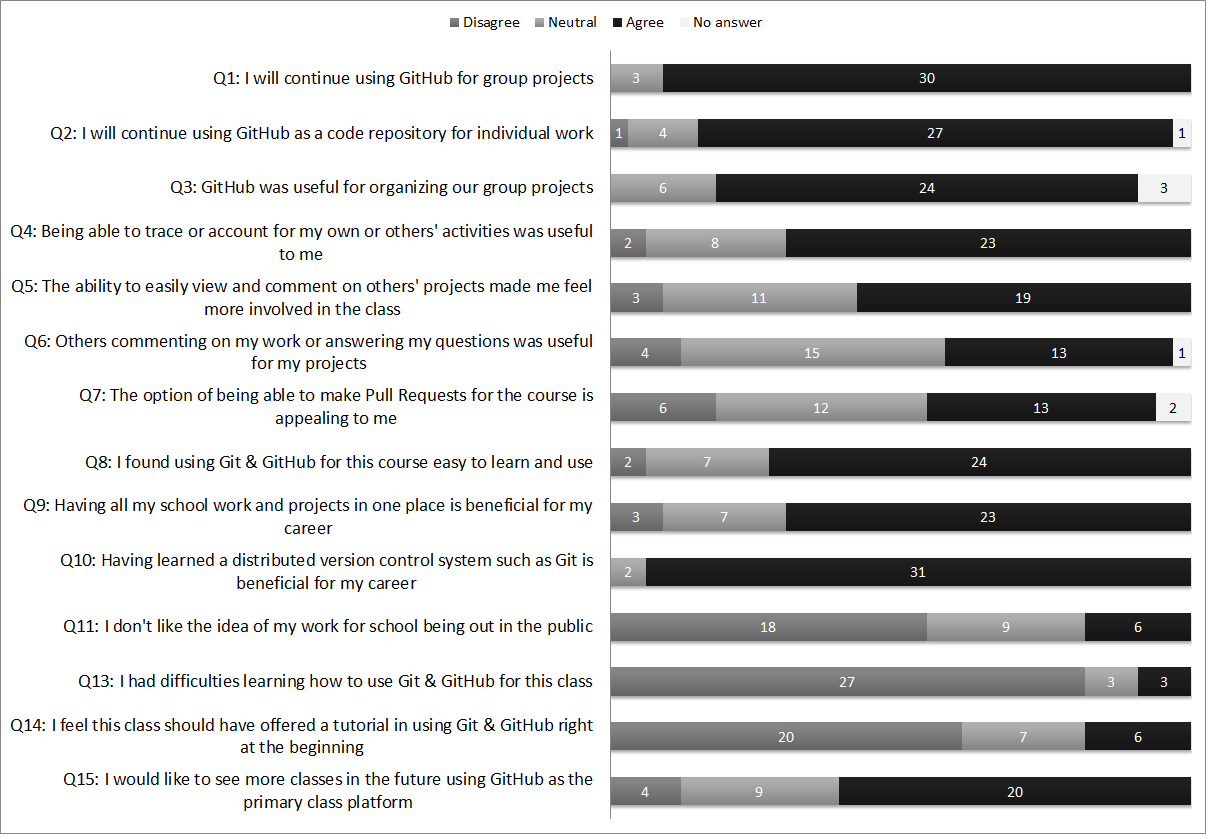
\includegraphics[width=0.75\textwidth]{surveychart}
\vspace{-4pt}
\caption{Aggregate of responses to validation survey questions}
\vspace{-12pt}
\end{figure*}

To validate the themes that emerged from the interviews, we sent a survey to all of the students in both courses at the end of the term (during the last week of the course). 33 students (18/34 DS and 15/29 SE) responded to the survey, giving us a response rate of 53\%.  The survey consisted of a set of Likert scale-style questions that were designed and pilot tested to confirm or refute our findings concerning the benefits and challenges students experienced.

Figure 1 provides a summary of the main questions we asked in the survey, as well as the responses we received.
As there were few differences between responses from the two different courses, we aggregate the responses shown in the figure (due to space limitations), but we discuss any notable differences between the two courses below.

In general, the survey validated the benefits and challenges that emerged from the interviews.
Of note is that 30 students (of the 33 that responded across both courses) agreed that they would \textbf{continue using GitHub} for group and individual work after the course concluded. Given that 14 of these students were completely or somewhat unfamiliar with GitHub before the course began, students seemed to believe that using GitHub can be beneficial for them outside of courses.
The majority of the students that responded also agreed that Git, GitHub, or other DVCSes should play a bigger role in their future courses and curriculum (20 agreed, 9 were neutral, and 4 disagreed).

In total, 19/33 students across both courses agreed that they were \textbf{more involved in the class} from viewing and commenting on other projects hosted on GitHub.
However, 11 of 15 SE respondents agreed, compared to only 8 of the 18 DS students who agreed.
This small difference may be due to the different levels of collaboration required across the two different courses, as the SE course required more collaboration in their lab assignments.

The survey also pointed to some divergences with the findings from the interviews.
From the interview responses, we expected that \textbf{privacy} was going to be a major concern to many students.
It was surprising to us that most students that responded to the survey from both courses disagreed or were neutral with the suggestion that their school work should not be publicly available.  This may be because the survey was conducted at the end of the term when their work was more polished and perhaps ready to be viewed by others.  Future work should consider this further.

Also, from the interviews, we expected that students would feel that a \textbf{tutorial} was necessary at the beginning of the course as they said they had trouble learning GitHub.  But in the survey, 20/33 (10 students from each course) disagreed that the classes needed a tutorial in the beginning of the semester.  This may have been because by the end of the term, students realized they could learn GitHub without such support.


% Not included because this is not discussed anywhere else in the paper.
%10 DS students disliked using the \emph{issues} as a discussion system on GitHub over forums with threaded discussions, while only 5 SE students disliked using GitHub `issues' for discussion.


%%% end of validation survey %%%

% section Findings (end)






%\subsection{Recommendations for Educators}
% \textbf{Recommendation: Utilize GitHub's Features} \\
%Computer science and software engineering students benefit from early exposure to Git and GitHub. By utilizing these (or similar) tools in their courses, educators provide students a way to familiarize themselves and practice with these tools, which can benefit their careers. Beyond exposure, hosting assignments, projects, and code on student accounts could be valuable when seeking employment, as companies continue to investigate the online presence prospective employees have (e.g., their GitHub accounts) for hiring purposes. x

%While simply using GitHub as a system for material dissemination can be helpful, using more of GitHub's features, such as pull requests and issues, provides even more benefits for the students. For example, allowing students to contribute to the course and to each other's work can help develop skills such as teamwork and communication \cite{hamer2006some}. For example, educators can use GitHub's transparency features to provide feedback to students in unique ways, such as tracing the history of student projects and assignments hosted on GitHub, detailing where students made mistakes and intervening when a student seems to be struggling. Moreover, in group projects, instructors can note how much work each student has contributed, and can use this transparency for assigning grades.

%As another example, exposure to GitHub's Issues feature, even for basic discussions, was helpful for one of the students interviewed during the second phase as the student learned how the feature works for use in future projects.

%One important lesson noted from the case study was to communicate the workflow the instructor decides clearly and properly to the teaching team and to the students. When deciding to use a feature like pull requests on course material, for example, the instructor must advertise this workflow properly, perhaps even offering bonus points for added material. To communicate a workflow to students and introduce GitHub and its features to novices, instructors should consider creating a guide or hosting a tutorial session. \\

%%%%%%%%%%%%%%%%%%%%%%%%%%%%%%%%%%%%%%
%Many students believed that GitHub worked best when a course has open-ended projects and assignments. This stems from plaigarism concerns that exist when students are putting their code up online where others can potentially see their solutions. Of course, students can submit their assignments in private repositories that only the instructors can view and contribute to. However, single-solution assignments being hosted in private repositories limit one of the most important benefits of using a system like GitHub---the ability to view, comment on, and contribute to the work of other students. As such, although GitHub can be used in any type of course, its benefits are maximized in courses with open-ended projects and courses where student contributions and participations. x

%; if the instructor creates a private repository for each student to submit their assignments and adds only the student as a collaborator, plaigarism would only be as much of a concern as it would be without using GitHub. Otherwise, an instructor could ask students to create a private repository for their assignments that only the instructors can view and contribute to.

% This style of repository management (where a private repository is dedicated to each student) could work for assignment submission as well. The instructor could ask the students to create a branch, or ask the students to fork off the main repositories and make the forks private, and then mandate that the student must make a pull request before a deadline. Thanks to GitHub's transparency features, an instructor can continuously observe the work in each student's repository and can provide further assistance to students based on the work history.

% However, the set up for this more private style of repository management requires some time and assistance from GitHub. An educator can create an organization for the course, which is granted an amount of private repositories depending on how much the instructor pays. While GitHub has stated that they would give teachers a free organization for their courses\footnote{\url{https://github.com/blog/1775-github-goes-to-school}}, an organization must be set up well before the course begins in order to get the private repositories in time.

 % As such, although GitHub is usable and helpful in any type of course, courses with open-ended projects and courses with a culture of participation are where instructors and students will see the primary benefits of using GitHub as a learning tool. If an instructor chooses to pursue the open-ended style of work similar to the courses in this study, it is recommended that they list projects and assignments on the home page using the readme markdown file so students can easily access the other projects.

% That said, GitHub continues to offer its benefits when used to submit single solution assignments. It involves some preparation to get free private repositories for students, but at the same time, it allows instructors to provide better feedback through versioning, and it maintains the benefits for students of learning Git and GitHub and hosting their work for future portfolio use (if allowed to publicize their work after the course concludes). \\

%contributions from others (slides in html, comment on other projects issues)
%Another recommendation is to encourage contribution from the students in the ways that GitHub affords them. First, students can contribute to the course materials by making corrections, changes, and adding resources. Second, students can contribute to other students' work and projects (provided the work is open-ended), bringing in an element of peer review that students may benefit from \cite{sondergaard2012collaborative}. And third, students can contribute to projects outside the course by making changes and pull requests in open-source repositories. Encouraging this `Contributing Student Pedagogy' can help students develop skills such as critical analysis and collaboration \cite{falkner2012supporting}.

% Moreover, all student contributions are available for the course instructor to see. As an example, an instructor can grade students based on their contributions, such as when they create an issue or a pull request on another project. However, one issue with student contributions that must be noted is that contributing to the course materials could present difficulties depending on the file types used, as binary files such as PDF documents and PowerPoint slides are not compatible with the GitHub web interface. Although GitHub has recently provided support for viewing PDF files on the platform\footnote{\url{https://github.com/blog/1974-pdf-viewing}}, these files remain unsupported by GitHub's `diff' feature, which means that changes to the file are difficult to discern and changes to the file by multiple people will always result in a `merge conflict'. For this reason, I recommend hosting class material and slides in either markdown or HTML, file types that GitHub supports and can be easily altered using its Web platform.
%%%%%%%%%%%%%%%%%%%%%%%%%%%%%%%%%%%%%%%%%%

%notifications

%!TEX root = icse_seet16.tex
\section{Discussion}
The motivation behind this study was to uncover student perceptions on using GitHub as an educational tool during the experience. GitHub was used in three main ways: (a) as a place to disseminate material and host the class schedule, (b) as a place for students to submit their lab assignments and discuss these assignments, and (c) as a place where most students interviewed hosted their course projects, either collaboratively or alone.

% \textbf{A Student-Oriented Learning Tool} \\
%What does GitHub provide? more opportunities for students to participate and contribute!

%accomplishing tasks related to some of the finer-grain features of traditional LMSes, such as a formal assignment submission, requires workarounds. E

% Where GitHub has the potential to excel, however, is in addressing some of the concerns regarding traditional LMSes outlined by various authors, such as the `walled garden` approach of traditional LMSes \cite{mott2010envisioning}. This could be addressed by giving students opportunities to participate in the course and connect with and learn from each other. GitHub can support these opportunities for students to become a part of each others' learning, creating a culture of participation \cite{jenkins2009confronting}. \\

\textbf{GitHub Supports the Contributing Student} \\
At a basic level, using GitHub for education can provide similar functions to those of traditional LMSes. As discussed in the last chapter, GitHub has the capabilities of providing many of the common activities found in Malikowski \textit{et al.}'s model of features found in LMSes \cite{malikowski2007model}. In the courses highlighted in this study, GitHub supported the two of the primary uses of LMSes from this model: information transmission and class discussions. However, even though GitHub can serve a similar purpose to formal educational tools, it was simply not built for education and is therefore lacking some educational features.

GitHub, however, can excel by providing opportunities for students to participate in their learning to create a culture of participation \cite{jenkins2009confronting}. Students are able to openly contribute to the course materials by making changes or additions directly to a course repository. Although only a few sutdents participated in contributing to the course material, many felt that this activity would have seen more use had it been advertised more. This plays a key role in Collis and Moonen's concept of a `Contributing Student' \cite{collis2006contributing}, where GitHub provides students the ability to drive their coursework. Moreover, the collaborative features of GitHub provides students simplified opportunities to partake in many of the `Contributing Student Pedagogy' activities Hamer \textit{et al.} described \cite{hamer2011tools}, including peer reviews, discussion, content construction, solution sharing, and making links.

When student assignments and projects are public, GitHub can provide students the opportunity to contribute to other students' learning by easily providing direct feedback to each other's assignments or project work. A number of groups in one of the courses in this study used this ability by leaving feedback for other groups when they noted bugs or issues in the code, and students appreciated this ability to see others' work and provide feedback as they saw fit. Contributing to other students' work may provide benefits in developing soft skills such as communication and teamwork skills \cite{hamer2006some}. As well, repurposing or remixing code can be a strong assessment tool for students due to practicality and prevention of plaigiarism \cite{sant2015code}. An instructor may also utilize GitHub to provide opportunities for students to peer review or grade each other's work. This could provide potential benefits such as more reflection for students while working, and the development of analysis and evaluation skills \cite{sondergaard2012collaborative}.

% However, it is important to note that like any technology, accessing these benefits requires the stakeholders to `buy in' and use the relevant features of the tool to support this pedagogy. It is possible, for example, that there were different levels of enthusiasm for the tool between the two courses because of the differences in how it was used in the lab sessions. The SE case required students to post often, which possibly encouraged them to look at others' responses, while the CS did not utilize the tool as much, requiring only a demo of the weekly assignments to the lab instructor instead.

\textbf{Transparency of Activities} \\
%accountability
In describing the benefits of using GitHub to support their group projects, some students described the transparency of activities as helpful for collaborating with each other. Few of the transparency features of GitHub were mentioned by the students---for example, the News Feed or the graphs were not discussed in the context of group projects. However, some students acknowledged the importance of seeing a history of work from other group members, describing the feature as a way to hold accountability and to keep up-to-date with the work, gaining the awareness that can be important in collaborative learning \cite{janssen2013coordinated}. This is in line with the benefits related to GitHub use in industry \cite{dabbish2012social}.

%better grading from instructors
Moreover, some students described the potential for better grading methods as a benefit of the transparency of activities on GitHub, despite these courses not utilizing the tool for grading. Compared to the traditional way of assignment submission where an assignment is handed in as a complete product when it is due, GitHub offers instructors the opportunity to monitor assignments and projects, giving feedback while they are in progress, a useful exercise for both parties \cite{glassy2006using}.

\textbf{Beyond the Course} \\
%practice in tool
Supporting the findings from interviews with early adopters of GitHub in education \cite{zagalsky2015emergence}, most of the students interviewed described being exposed to GitHub and its features as a benefit to using the tool in a course. As such, the exposure to GitHub and its open, collaborative workflow may result in some transferable skills towards their careers. Moreover, the popularity of the tool means that students' GitHub accounts become part of their online presence \cite{marlow2013impression}, which may serve an important role with future collaborators or potential employers who use GitHub for hiring purposes.

%outside help
With GitHub's popularity, many developers are putting their code on the platform, both publicly or privately. When a course is publicly visible, the `walled garden' that traditional LMSes tend to suffer from \cite{mott2010envisioning} can be overcome. Student projects, for example, could involve people from another community, or outsiders can contribute to the course materials in some manner. \\

% \textbf{Tool Literacy} \\
% %privacy issues
% An important note from some of the limitations that the students and the instructors described is the importance of understanding and being proficient with the tool. As an example, in discussing what considerations need to be made to design an effective workflow, students would discuss the difficulty of conducting courses with single-solution assignments rather than open-ended projects. This was due to the way in which GitHub repositories are required to be private or public, making it difficult to handle assignment submission.
%
% However, some experience with the tool or some investigation of GitHub's recommended practices for using their tool in education would have revealed the possibility of using private repositories for each assignment. An instructor could introduce new assignments or make clarifications in a student's private repository if they were simply added as a collaborator. As such, it is important to consider that some of the limitations described by the students and by the instructor may be from unfamiliarity with using the tool, especially in a context it originally was not meant to serve.

%opportunistic
%group interviews
\subsection{Threats to Validity}
In this section, we discuss the threats to validity of our research.

\subsubsection{Internal Validity}
Internal validity is concerned with biases within a study that might affect our results \cite{creswell2013research}. In our research, the recruitment methods may have biased the population: by searching for instructors teaching appropriate courses, we first approached instructors we knew to invite them to participate in our study, which may have limited the study in comparison to finding a professor who was already intending to use GitHub as a learning tool and had experience in doing so. As well, opportunistic recruitment of the students may have resulted in a situation where the students willing to be interviewed were students who felt strongly about GitHub in either direction---those who may have had insights but had no strong opinions may have chosen not to participate. By interviewing many students however, we were able to discover any contradictions or discrepancies between them.

The data analysis also threatens the validity of the study as there was no inter-rater reliability because there was one coder. As such, biases may have been introduced in the selection of the themes. Having multiple raters analyze the data would have introduced more perspectives and interpretations, which would have reduced the potential biases in the analysis. The validation survey, however, mitigated some of the potential bias this limitation introduces, as the survey served as a form of member checking, allowing students to verify the analysis of the data.

\subsubsection{External Validity}
 External validity is concerned with the extent to which the findings from this work can be generalized and to what extent the findings are of interest to people outside the case \cite{runeson2012case}. As a case study, it cannot be assumed that these cases can be generalized to the use of GitHub in education. In particular, because of the instructor's lack of experience with using GitHub, these findings may vary from courses in which the instructor was able to offer more guidance with using the tool. However, many of the findings are reflected in other studies that use similar tools for classes, such as Kelleher's study on Git and GitHub \cite{kelleher2014employing}, and Haaranen and Lehtinen's study on Git and GitLab \cite{haaranen2015teaching}.

%However, we used a number of approaches\cite{runeson2012case} to establish rigor and to minimize the threats to validity described above. One such approach included triangulating data from multiple students. In doing so, we able to identify and highlight contradictions between students. Moreover, we deployed a survey to students in both courses in order to validate the themes extracted from the interviews. This is a form of member checking and allows students to verify the analysis of the data. %Finally, this study also involved a peer with whom I discussed the study with regularly. This peer, who is experienced with qualitative research methods, was consulted throughout the study, including the study design and the collection and analysis of data, and would lower the risk of any biases affecting the study.

%This resulted in a less than optimal use of GitHub (as described by many of the students interviewed) because the instructor had little prior experience with GitHub as a tool. As well, because of this inexperience, the researchers would give the instructor advice or resources on possibilities of how they can use GitHub to meet a goal---we didn't, however, directly give them step-by-step directions to avoid influencing the direction of the class as much as possible.

% In the data analysis, there was no inter-rater reliability because I was the sole coder. As such, biases may have been introduced in my selection of the themes. Having multiple raters analyze the data would have introduced more perspectives and interpretations, which would have reduced the potential biases in the analysis. Unfortunately, this study suffers from a single-rater limitation.

%As well, the opportunistic nature of recruitment may have resulted in possible biases in multiple ways. With only one instructor teaching two courses, this study is limited from having no other cases to compare with, particularly cases where the instructor might be experienced with using GitHub.

% However, we used a number of approaches\cite{runeson2012case} to establish rigor and to minimize the threats to validity described above. One such approach included triangulating data from multiple sources---the students as well as the teaching team. In doing so, I was able to identify and highlight contradictions between different sources and report discrepant information.
%
% This study was also conducted over the span of the two courses which provided prolonged involvement with the population and allowed for a good understanding of the participants' perspectives. Moreover, we deployed a survey to students in both courses in order to validate the themes extracted from the interviews. This is a form of member checking and allows students to verify the analysis of the data. %Finally, this study also involved a peer with whom I discussed the study with regularly. This peer, who is experienced with qualitative research methods, was consulted throughout the study, including the study design and the collection and analysis of data, and would lower the risk of any biases affecting the study.

%In summary, this study has shown the effectiveness of using GitHub for educational purposes from the student perspective. This study describes the benefits of using GitHub for education, such as the possibilities for student contributions. However, these benefits are accompanied by limitations, such as the implications of having publicly available work on cheating and academic integrity. In the next chapter, I offer recommendations for instructors who want to attempt using GitHub in their courses in order to maximize the benefits of using the tool.

\section{Conclusion}

%Limitations

%Future Work

%Contributions
Another important consideration from this work relates to the future of tools for computer science and software engineering education---what's next? First, we consider the importance of participation, group work, and group learning for students in technical fields in order to develop non-technical `soft' skills such as communication and teamwork \cite{jazayeri2004education}. This work demonstrates how using GitHub can unlock activities where students can contribute to each other's learning, and as a result, I believe it can be beneficial to add support for GitHub's open, collaborative workflow to current and future tools focused on learning.

%GitHub for Education
% The fact that GitHub easily supports participatory activities has multiple implications. Literature has shown that LMSes have been adding `Web 2.0' features such as blogs and wikis to their feature set \cite{downes2005feature}---students are being offered more opportunities to participate by discussion or by contributing content in blogs or wikis. Where the GitHub Way excels in education, however, is in the opportunities for students to contribute to and change the materials, and to contribute to each other's learning by getting involved in and providing feedback to projects other than their own. This is potentially the next step for Learning Management Systems, where students are more easily able to make these contributions to the work of others. The concern, however, is that implementing features similar to GitHub in an LMS might seem forced and haphazardly planned, and tool builders would be better served building a tool that supports and encourages an open, collaborative workflow from the outset.

As such, one possible path is the `GitHub for Education' Greg Wilson discussed\footnote{\url{http://software-carpentry.org/blog/2011/12/fork-merge-and-share.html}}, where a tool like GitHub can be altered or built to be more focused towards education. The main weakness of GitHub when used in this context is in the lack of flexibility in its privacy and in the lack of administrative functions such as gradebooks and announcements. Meanwhile, there are open-source alternatives to GitHub such as GitLab\footnote{\url{https://about.gitlab.com}}, that could be further developed into a tool that fulfils more educational needs. As an example, it could be valuable to implement a form of announcements, a notification feature that students have more control over, and a way to make some discussions or issues within a repository private while others remain public. This is potentially an avenue for future work, where such a tool can be evaluated.

% As well, because of the exploratory nature of the work, we sought to obtain teacher and student perspectives regarding just the viability of GitHub as a tool for education. However, other studies have investigated using tools such as wikis \cite{minocha2007collaborative} and how they possibly affect or correlate with student performance. This is one natural extension of this work: running a field experiment to see whether or not using the tool simply engages the students more or if it can ultimately affect grades.

In summary, this work has shown the viability of using GitHub for education, and has demonstrated why the open, collaborative workflow associated with GitHub should be considered when deciding which tools to use to support a course. Based on the findings of this work, we included a set of recommendations for educators interested in using GitHub as a learning tool, and list the implications on tools that could provide the same benefits as GitHub while mitigating the limitations.


%ACKNOWLEDGMENTS are optional
%\section{Acknowledgments}

%
% The following two commands are all you need in the
% initial runs of your .tex file to
% produce the bibliography for the citations in your paper.
\bibliographystyle{abbrv}
\bibliography{icse_seet16}  % sigproc.bib is the name of the Bibliography in this case
% You must have a proper ".bib" file
%  and remember to run:
% latex bibtex latex latex
% to resolve all references
%
% ACM needs 'a single self-contained file'!
%

%\balancecolumns % GM June 2007
% That's all folks!
\end{document}
